\graphicspath{{0_FrontMatter/Figures/}}

\begingroup
\setlength{\parindent}{0pt}

%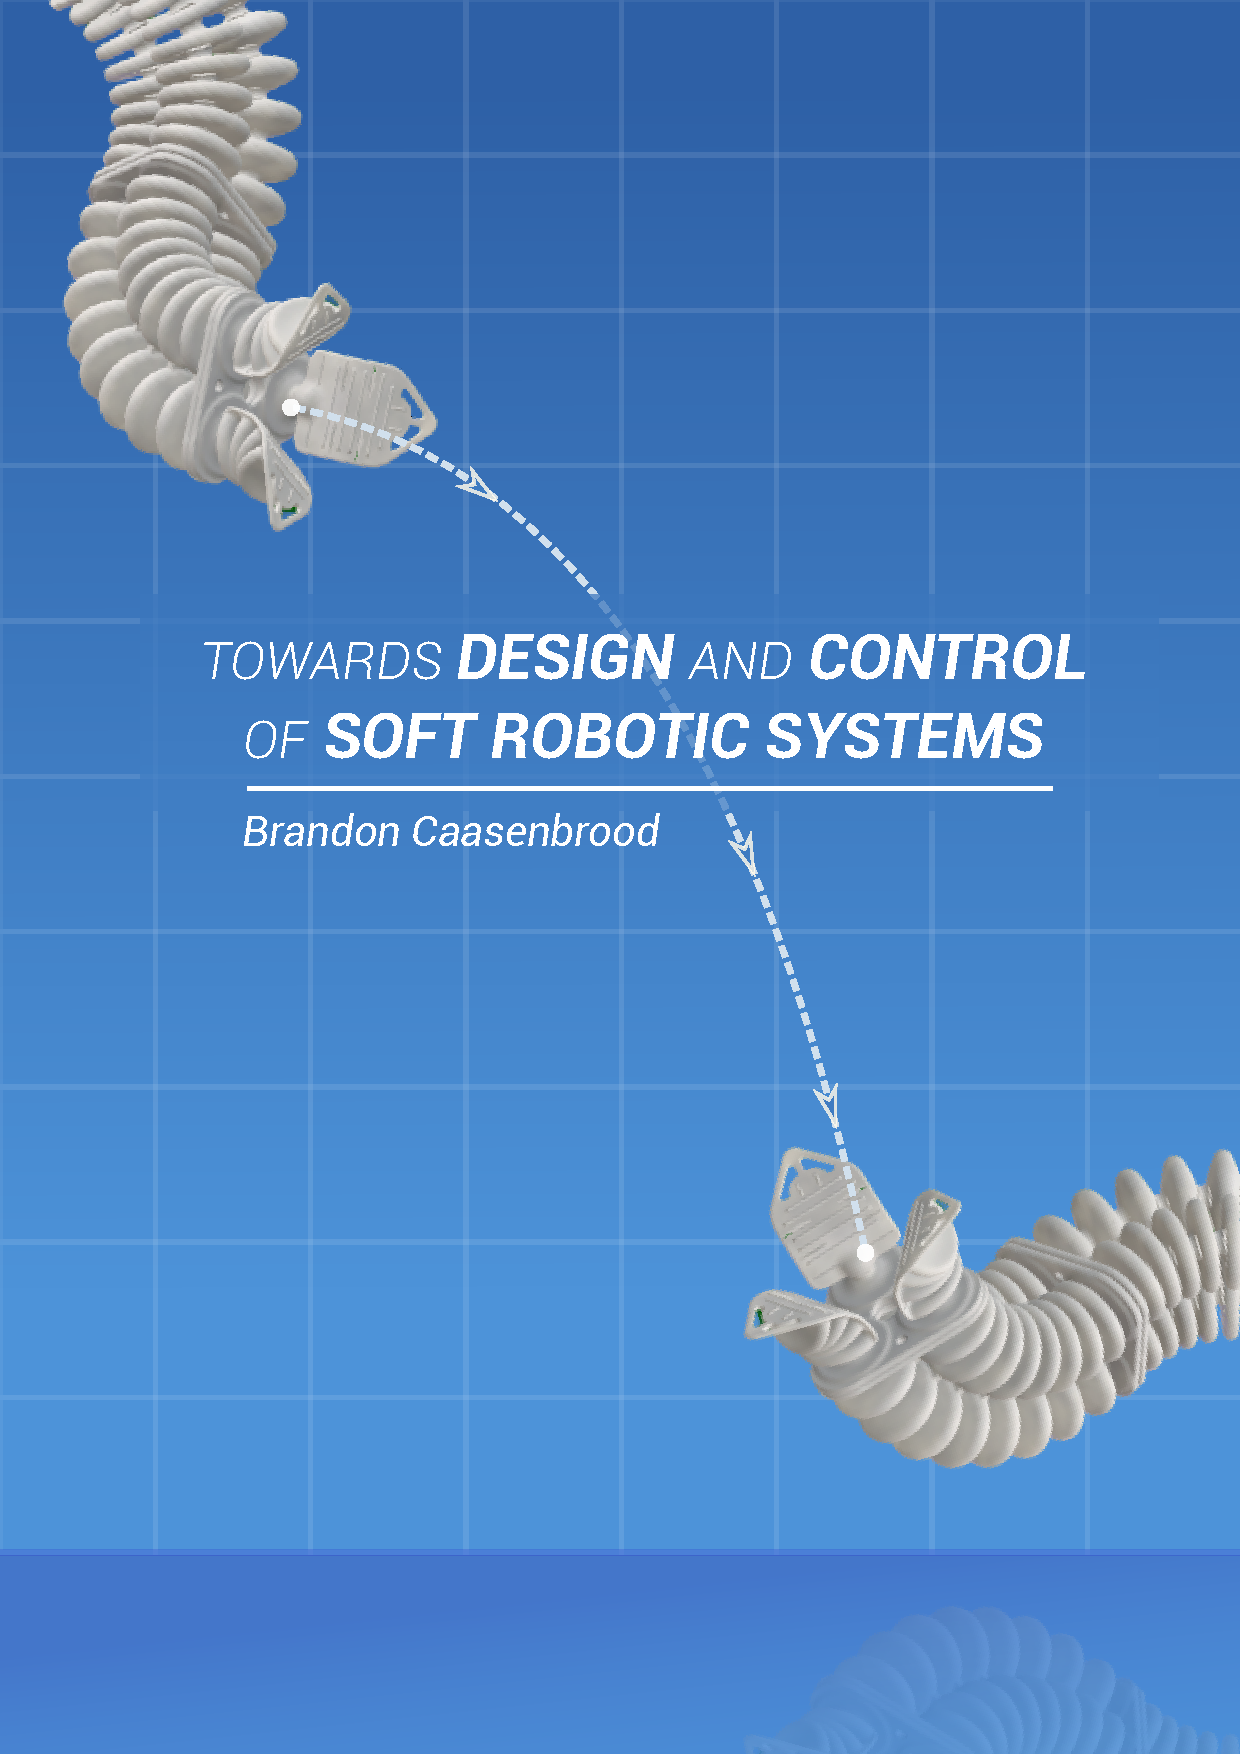
\includepdf[page=1]{./cover/cover-1.pdf}
%%%%%%%%%%%%%%%%%%%%%%%%%%%%%%%%%%%%%%%%%%%%%%%%%%%%%%%%%%%%%%%%%%%%%%%%%%%%%%%%%%%%%%%%%%%%%%%%%%%%%%%%%%%%%%%%%%%%%%%%%%%%%%%%%%%%%%%%%%%%
\thispagestyle{empty}
\vspace*{3cm}
\begin{center}
\iftuefont
\huge{\tuefontscala\selectfont\maintitle}\\[15mm]%[30mm]%[3mm]
%\Large{\tuefontscala\selectfont\subtitle}\\[30mm]
\Large{\tuefontscala\selectfont Brandon Jonathan Caasenbrood}
\else
\huge{\sffamily\bfseries\selectfont\maintitle}\\[15mm]%[30mm]%[3mm]
%\Large{\sffamily\selectfont\subtitle}\\[30mm]
\Large{\sffamily\selectfont Camiel Beckers}
\fi
\end{center}

%%%%%%%%%%%%%%%%%%%%%%%%%%%%%%%%%%%%%%%%%%%%%%%%%%%%%%%%%%%%%%%%%%%%%%%%%%%%%%%%%%%%%%%%%%%%%%%%%%%%%%%%%%%%%%%%%%%%%%%%%%%%%%%%%%%%%%%%%%%%
\newpage
\thispagestyle{empty}
\textbf{About the cover}
**Explanation**\\
{\footnotesize Photo: ??}

\vspace*{\fill}

%
\includegraphics[height=1.5cm,trim={3mm 3mm 0 0},clip]{0_FrontMatter/Figures/TUe-logo-descriptor-line-scarlet-cmyk}\\[3mm]
%{\small The work described in this thesis was carried out at the Eindhoven University of \linebreak Technology.}\\[5mm]

%
\includegraphics[height=9mm]{disclogo.pdf}
%\\[2mm]
%{\small
%The author has successfully completed the educational program of the Graduate School of the Dutch Institute of Systems and Control (DISC).}\\


\includegraphics[height=1.35cm]{TUe-logo-descriptor-line-tight}
\\[4mm]
{\small
The work described in this thesis was carried out at the Eindhoven University of Technology (TU/e).
\\[2mm]
A catalogue record is available from the Eindhoven University of Technology Library.\\
ISBN: ??
\\[3mm]
Typeset with \LaTeX.
\\
Cover design by ??
\\
Reproduction by ??
%\\[3mm]
\\[2mm]
\vspace{0.64854cm}
***FSC keurmerk hier***
%\cbox{FSC}\vspace{0.64854cm} %1cm-0.35146cm= 1cm-em
%\includegraphics[height=1.25cm]{FSC_logo} % FSC figures have a unique code
%\\[3mm]
\\[2mm]
%Cover photo: freepik.com/wirestock. For further information, see [\Cancer] on page \pageref{covernote}.\\[3mm]
\copyright\,2021 by ??. All rights reserved.}


%%%%%%%%%%%%%%%%%%%%%%%%%%%%%%%%%%%%%%%%%%%%%%%%%%%%%%%%%%%%%%%%%%%%%%%%%%%%%%%%%%%%%%%%%%%%%%%%%%%%%%%%%%%%%%%%%%%%%%%%%%%%%%%%%%%%%%%%%%%%
\newpage
\thispagestyle{empty}
\begin{otherlanguage}{dutch}

\vspace*{\fill}

\begin{center}
\iftuefont
\huge{\tuefontscala\selectfont \maintitle}\\[30mm]
\else
\huge{\sffamily\selectfont \maintitle}\\[30mm]
%\huge{\sffamily\selectfont \maintitle}\\[3mm]
\fi
%\Large\subtitle\\[30mm]
\normalsize {PROEFSCHRIFT}\\[8mm]
ter verkrijging van de graad van doctor aan de\\
Technische Universiteit Eindhoven, op gezag van de\\
rector magnificus prof.dr.ir. F.P.T. Baaijens, voor een\\
commissie aangewezen door het College voor\\
Promoties, in het openbaar te verdedigen\\
op ??dag ?? ?? 2022 om ??.00 uur\\[8mm]
door\\[8mm]
??\\[8mm]
geboren te ??
\end{center}

\vspace*{\fill}


%%%%%%%%%%%%%%%%%%%%%%%%%%%%%%%%%%%%%%%%%%%%%%%%%%%%%%%%%%%%%%%%%%%%%%%%%%%%%%%%%%%%%%%%%%%%%%%%%%%%%%%%%%%%%%%%%%%%%%%%%%%%%%%%%%%%%%%%%%%%
\newpage
\thispagestyle{empty}
Dit proefschrift is goedgekeurd door de promotoren en de samenstelling van de promotiecommissie is als volgt:\\[\baselineskip]
\begin{tabular}{@{}ll}
voorzitter:	& ??\\
1\textsuperscript{e} promotor:	& ??\\
2\textsuperscript{e} promotor:	& ??\\
%copromotor:						& ***\\
leden:		& ??\\
			& ??\\
			& ??\\
			& ??\\
			& ??\\
adviseur:	& ??
\end{tabular}

\vspace*{\fill}

\begin{flushleft}
Het onderzoek dat in dit proefschrift wordt beschreven is uitgevoerd in overeenstemming met de TU/e Gedragscode Wetenschapsbeoefening.
\end{flushleft}

\end{otherlanguage}

% Epigraph
\clearpage
\thispagestyle{empty}

\vspace*{\fill}

\begin{center}
  Epigraph
\end{center}

\vspace*{\fill}

\endgroup
